\documentclass[12pt]{standalone}
\usepackage{amssymb,amsmath}
\usepackage{tikz}
\usetikzlibrary{fit,shapes.multipart}
\usetikzlibrary{shapes, arrows, calc, positioning,arrows.meta,decorations.markings,math}
\usetikzlibrary{decorations.pathreplacing}
\usepackage{xcolor}
\usepackage{pgfplots}
\usepackage[most,listings]{tcolorbox}
\usepackage{bm}
\usepackage[outline]{contour}
\contourlength{1.2pt}


\usetikzlibrary{fit,shapes.multipart}
\usetikzlibrary{shapes, arrows, calc, positioning,arrows.meta,decorations.markings,math}
\usetikzlibrary{decorations.pathreplacing}

\renewcommand{\familydefault}{\sfdefault}

\definecolor{dBlue}{RGB}{0,166,235}
\definecolor{xDarkBlue}{RGB}{11,21,70}
\definecolor{xOrange}{RGB}{243,146,0}
\definecolor{xDarkBox}{RGB}{129,176,200}
\definecolor{xDarkItem}{RGB}{85,157,187}
\definecolor{xLightBox}{RGB}{227,235,242}


\tcbset{on line,arc=0.5cm,
  boxsep=4pt, left=0pt,right=0pt,top=-4pt,bottom=0pt,
  colframe=white,colback=xLightBox,  
  highlight math style={enhanced}
}
\newcommand{\sca}{\widehat{\rho}}
\newcommand{\ft}{\mathcal{F}}
\newcommand{\ift}{\mathcal{F}^{-1}}
\begin{document}

  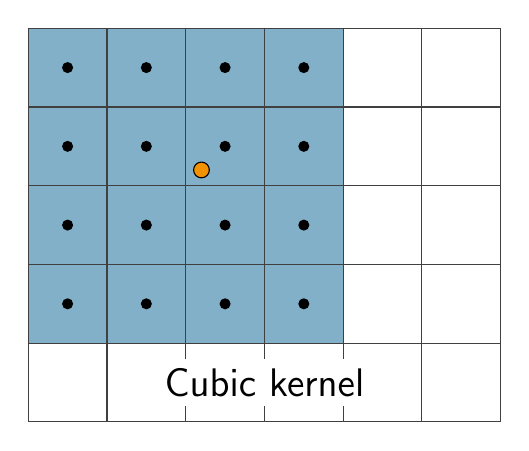
\begin{tikzpicture}
    % Fill one square in orange
    \fill[xDarkBox] (0,1) rectangle (4,5);
    %\fill[xLightBox] (1.5,1.5) rectangle (4.5,4.5);

    \fill[xOrange,draw=black] (2.2,3.2) circle (0.1);
    
    \begin{scope}[shift={(0.5,0.5)}]
        %\draw[step=1cm, black, dashed] (-1,-1) grid (6,5);
        \foreach \x in {0,...,3} {
          \foreach \y in {1,...,4} {
            \fill (\x,\y) circle (2pt);
          }
        }
    \end{scope}
    \draw[step=1cm, darkgray] (0,0) grid (6,5);
    \node[fill=white] (label) at (3,0.5) {\Large Cubic kernel};
    
  \end{tikzpicture}

\end{document} 
